\documentclass[11pt, oneside]{article}   	% use "amsart" instead of "article" for AMSLaTeX format
\usepackage{geometry}                		% See geometry.pdf to learn the layout options. There are lots.
\geometry{letterpaper}                   		% ... or a4paper or a5paper or ... 
%\geometry{landscape}                		% Activate for for rotated page geometry
%\usepackage[parfill]{parskip}    		% Activate to begin paragraphs with an empty line rather than an indent
\usepackage{graphicx}				% Use pdf, png, jpg, or eps� with pdflatex; use eps in DVI mode
								% TeX will automatically convert eps --> pdf in pdflatex		
\usepackage{amssymb}
\usepackage{amsmath}
\usepackage{parskip}
\usepackage{color}
\usepackage{hyperref}

\title{notes}
%\author{The Author}
%\section{}
%\subsection*{}
\date{}							% Activate to display a given date or no date

\graphicspath{{/Users/telliott_admin/Dropbox/Tex/png/}}
% \begin{center} 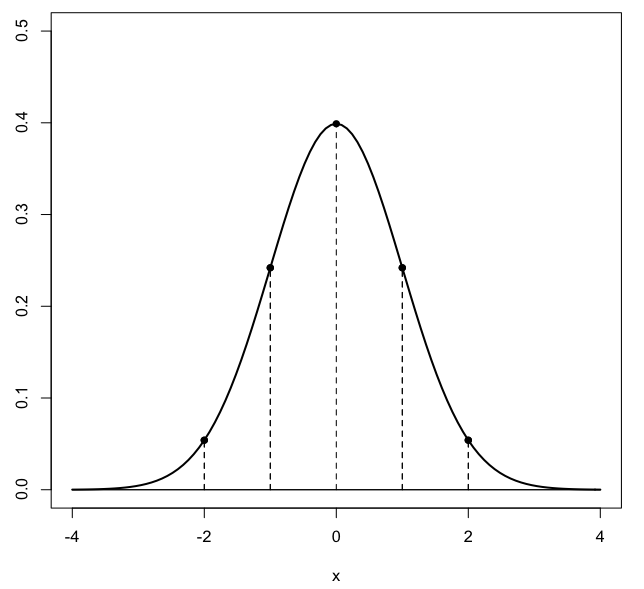
\includegraphics [scale=0.4] {gauss3.png} \end{center}
\begin{document}
\maketitle
\Large
I ran into what looks like a funky field this morning in a Calc 3 book.  Consider:
\[ f(x,y) = \theta \]
where $\theta$ is, as usual, the angle corresponding to that formed by the ray reaching out to the point in polar coordinates.
\[ \theta = \tan^{-1} \frac{y}{x}, \ \ \ \ -\frac{\pi}{2} < \theta < \frac{\pi}{2} \]
Now compute
\[ \mathbf{F} = \nabla f = \ \langle \ \frac{\partial f}{\partial x}, \frac{\partial f}{\partial y} \ \rangle \]
To pre-compute a bit, the derivative of $\tan^{-1} t$ is $1/(1+t^2)$, so our derivatives will both have a factor of
\[ \frac{1}{1 + y^2/x^2} = \frac{x^2}{x^2 + y^2} \]
The derivatives are then what we have above times the derivative of the argument to $\tan^{-1}$:
\[ \frac{\partial}{\partial x} \ \tan^{-1} \frac{y}{x} = \frac{x^2}{x^2 + y^2} \cdot (\frac{-y}{x^2} ) = \frac{-y}{x^2 + y^2}\]
\[ \frac{\partial}{\partial y} \ \tan^{-1} \frac{y}{x} = \frac{x^2}{x^2 + y^2} \cdot \frac{1}{x} = \frac{x}{x^2 + y^2} \] 
\[ \mathbf{F} = \frac{1}{x^2+y^2} \ \langle \  -y, x\ \rangle \]
\subsection*{line integral}
Now, since $\mathbf{F}$ is the gradient of a potential function you might expect that the line integral around a closed path will be zero.

If we are just presented with $\mathbf{F}$, not knowing anything else, one test to do is to compute the mixed partials and see if they are equal.  That is, we should compute:
\[ M_y = \frac{d}{dy} \ \frac{-y}{x^2 + y^2} = \frac{-(x^2 + y^2) + 2 y^2}{(x^2 + y^2)^2} = \frac{y^2 - x^2}{(x^2 + y^2)^2} \]

\[ N_x = \frac{d}{dx} \ \frac{x}{x^2 + y^2} = \frac{(x^2 + y^2) - 2x^2}{(x^2 + y^2)^2} = \frac{y^2 - x^2}{(x^2 + y^2)^2} \]
The theorem is that \emph{if} the mixed partials are not equal, then the field is not conservative.  The converse is also true, but has an additional requirement, as we will see.  Let's compute the line integral.
\[ \oint M \ dx + N \ dy \]
That factor of $x^2 + y^2$ makes me think polar coordinates should be the way to go (not to mention that we started with $f(x,y) = \theta$).  Let's take the unit circle centered at the origin as the path, going counter-clockwise.
\[ x = \cos \theta \]
\[ dx = - \sin \theta \ d \theta \]
\[ y = \sin \theta \]
\[ dy = \cos \theta \ d \theta \]
\[ x^2 + y^2 = \cos^2 \theta + \sin^2 \theta = 1 \]
\[ M = \frac{-y}{x^2 + y^2}  = - \sin \theta \]
\[ N = \frac{x}{x^2 + y^2} = \cos \theta \]
So
\[ \oint M \ dx + N \ dy = \oint \sin^2 \theta \ d \theta + \cos^2 \theta \ d \theta  \]
\[ = \oint d \theta = \theta \ \bigg |_0^{2 \pi} = 2 \pi \]
Indeed the integral around this closed path is \emph{not} zero and the field is not conservative.  Why not?

The additional requirement that we skirted around above is that the field must be defined everywhere in the region inside the closed curve.  But neither component of $\mathbf{F}$ is defined at the origin.  Somehow, that deficiency makes it blow up and give a non-zero integral on this path.

It is also worth pointing out that if the path does not include the origin, then the field \emph{is} conservative and the integral will be zero.  

\subsection*{path not including the origin}

Suppose we go around the displaced unit square starting from $(1,0)$.  The region is $[1,2] \times [0,1]$.

$C1$:   $y=0$, $dy = 0$
\[ \int_1^2 M \ dx = \int_1^2  \frac{-y}{x^2 + y^2} \ dx =  \int_1^2 0 \ dx = 0 \]

$C2$:   $x=2$, $dx = 0$
\[ \int_0^1 N \ dy = \int_0^1  \frac{x}{x^2 + y^2} \ dy =  \int_0^1 \frac{2}{4 + y^2} \ dy  \]
Leave aside the factor of $2$ for a moment.  

The basic integral is $1/a + y^2$, which we deal with by substitution:  $\sqrt{a} u = y$, $au^2 = y^2$ and $\sqrt{a} \ du = dy$ so
\[ \int \frac{1}{a + y^2} \ dy = \sqrt{a} \int \frac{1}{a + au^2} \ du = \frac{1}{\sqrt{a}} \int \frac{1}{1 + u^2} \ du \] 
\[ = \frac{1}{\sqrt{a}} \ \tan^{-1} u = \frac{1}{\sqrt{a}} \ \tan^{-1} \frac{y}{\sqrt{a} } \]
We have the same bounds, because we have switched back to $y$ as the variable.  Recall the factor of $2$ and that $a = 4$ so we have
\[ = 2 \cdot \frac{1}{2} \tan^{-1} \frac{y}{2} \ \bigg |_0^1 = \tan^{-1} \frac{1}{2} \]
Let's leave it in this form for now.

$C3$:   $y=1$, $dy = 0$
\[ \int_2^1 M \ dx = \int_2^1  \frac{-y}{x^2 + y^2} \ dx = \int_2^1  \frac{-1}{1 + x^2} \ dx \]
\[ = \int_1^2  \frac{1}{1 + x^2} \ dx = \tan^{-1} 2 - \tan^{-1} 1  \]
$C4$:  $x=1$, $dx = 0$
\[ \int_1^0 N \ dy = \int_1^0 \frac{x}{x^2 + y^2} \ dy = \int_1^0 \frac{1}{1^2 + y^2} \ dy \]
\[ = \tan^{-1} 0 - \tan^{-1} 1 \]
So, all together we have:
\[ \tan^{-1} \frac{1}{2} + \tan^{-1} 2 - 2 \tan^{-1} 1 \]
Now, the angles whose tangents are equal to $1/2$ and $2$ ($\approx 63$ degrees) are not exactly nice, but they are complementary angles and so the sum is equal to $\pi/2$, which \emph{is} nice.  The angle whose tangent is equal to $1$ is, of course, $\pi/4$.  So 
\[ \frac{\pi}{2} - 2 \ \frac{\pi}{4} = 0 \]
Everything cancels and the final result is just $0$.  This field is conservative and the line integral around a closed path is equal to zero, as long as that path does not enclose the origin.

I suppose we could think about a circle of radius $1$ displaced from the origin to $(2,0)$.  But I ran into trouble trying to calculate that one.

It is also worth pointing out that conservation fails if we even just touch the origin on the curve.  Consider the part of the unit circle in the first quadrant.  The integral from $x=0 \rightarrow 1$ is zero since $y=0$ and $dy=0$ and so is the other part coming back along the $y$-axis.  But the integral over the arc is $\pi/2$.  So the total is not zero.

And now that I think about it, suppose we complete the closed curve, not by going back to zero, but by following some other path.  We must have zero for the whole path, and that means that the integral along \emph{any} path from the positive $y$-axis to the positive $x$-axis excluding the origin is $- \pi/2$.

\end{document}  